\documentclass{beamer}
\setbeamertemplate{footline}[frame number]
%\documentclass{beamer}

\usepackage[utf8x]{inputenc}
\usepackage[brazil,british]{babel}
\usetheme{default} 
\usecolortheme{beaver}
\newtranslation[to=brazil]{Theorem}{Teorema}
\newtranslation[to=brazil]{Definition}{Definição}
\newtranslation[to=brazil]{Example}{Exemplo}
\newtranslation[to=brazil]{Problem}{Exercício}
\newtranslation[to=brazil]{Solution}{Resolução}
\logo{
\includegraphics[width=1cm]{../img/logo-ppgsc-icon-text.png}}

\usepackage{graphicx}
\usepackage{clrscode3e}
\usepackage{hyperref}

\usepackage{pgf}
\usepackage{tikz}
\newcommand{\assert}[1]{\textcolor{blue}{#1}}



\usepackage{tikz}
\usetikzlibrary{arrows,positioning, calc} 
\tikzstyle{vertex}=[draw,fill=black!15,circle,minimum size=18pt,inner sep=0pt]

\title{Aula 13: Estruturas de dados básicas, parte 1}
\author{David Déharbe \\
  Programa de Pós-graduação em Sistemas e Computação \\
  Universidade Federal do Rio Grande do Norte \\
  Centro de Ciências Exatas e da Terra \\
  Departamento de Informática e Matemática Aplicada}
\date{30 de março de 2015}


\begin{document}
\selectlanguage{brazil}
\begin{frame}
  \titlepage
  Download me from \url{http://ufrn.academia.edu/DavidDeharbe}.
\end{frame}

\begin{frame}
  \frametitle{Plano da aula}
  \tableofcontents
\end{frame}

\section{Introdução}

\begin{frame}
  \frametitle{Motivação}

  \begin{itemize}
  \item Diferentes aplicações computacionais utilizam
    matrizes e álgebra linear para modelar e calcular
    \begin{itemize}
      \item previsão do tempo
      \item engenho de busca
      \item jogos
      \item análise estática de programas
      \item etc.
    \end{itemize}
  \item Como representar uma matriz?
    \pause
    \begin{itemize}
      \item \alert{arranjo de arranjos}
      \item \alert{lista encadeada} das entradas não nulas de cada linha e de
        cada coluna.
    \end{itemize}
  \item Qual a melhor forma?
    \pause
    Assume matrizes de dimensão $n$, sendo que a probabilidade de uma 
    entrada ser 0 é $p$. Calcule:
    \begin{itemize}
      \item Quantidade de espaço utilizado
      \item Custo da multiplicação de duas matrizes
    \end{itemize}
    $T_n$ e $T_p$ são o tamanho da representação de um número e
    de um ponteiro.
  \end{itemize}

\end{frame}

\begin{frame}
  \frametitle{Caracterização}

  Ref: Cormen et al. Capítulo 11.
  
  Como implementar uma coleção homogênea de dados?
  \begin{itemize}
  \item \alert{coleção} conjunto de dados armazenados
  \item Evolução dinâmica do conjunto armazenado
  \item \alert{homogênea} todos os dados têm um mesmo tipo
  \item Todos os dados possuem uma \alert{chave}
  \item Relação de ordem entre chaves
    $$
    \forall x, y \cdot x < y \lor x > y \lor x = y
    $$
  \item Estrutura entre os dados
  \item Operações disponíveis e seu custo
  \end{itemize}

\end{frame}

\begin{frame}

  \frametitle{Tipos e operações básicas}

  \begin{description}
    \item[tipos]
      \begin{itemize}
        \item chave
        \item dado
        \item coleção
        \item posição na coleção (iterador)
      \end{itemize}
    \item[operações]
      \begin{itemize}
        \only<2>{
        \item \alert{busca} chave em coleção, retorna posição
          \begin{itemize}
            \item da primeira ocorrência, ou
            \item da primeira ocorrência a partir da posição dada, ou
            \item da próxima ocorrência desde a última busca.
          \end{itemize}
        }
        \only<3>{
        \item \alert{insere} chave em coleção, 
          \begin{itemize}
            \item depois da posição dada, ou
            \item antes da posição dada, ou
            \item na posição correspondente ao invariante.
          \end{itemize}
        }
        \only<4>{
        \item \alert{remove} elemento da coleção
          \begin{itemize}
            \item na posição dada, ou
            \item com a chave dada, ou
            \item o elemento correspondente ao invariante.
          \end{itemize}
        }
        \only<5>{
        \item \alert{menor} elemento da coleção.
        \item \alert{maior} elemento da coleção.
        }
        \only<6>{
        \item posição \alert{inicial} na coleção.
        \item posição \alert{final} na coleção.
        \item posição \alert{seguinte} à posição dada na coleção.
        \item posição \alert{anterior} à posição dada na coleção.
        \item \alert{n-ésima} posição na coleção.
        }
      \end{itemize}
  \end{description}
\end{frame}

\section{Pilhas}

\begin{frame}
  \frametitle{Pilhas}

  \begin{center}
    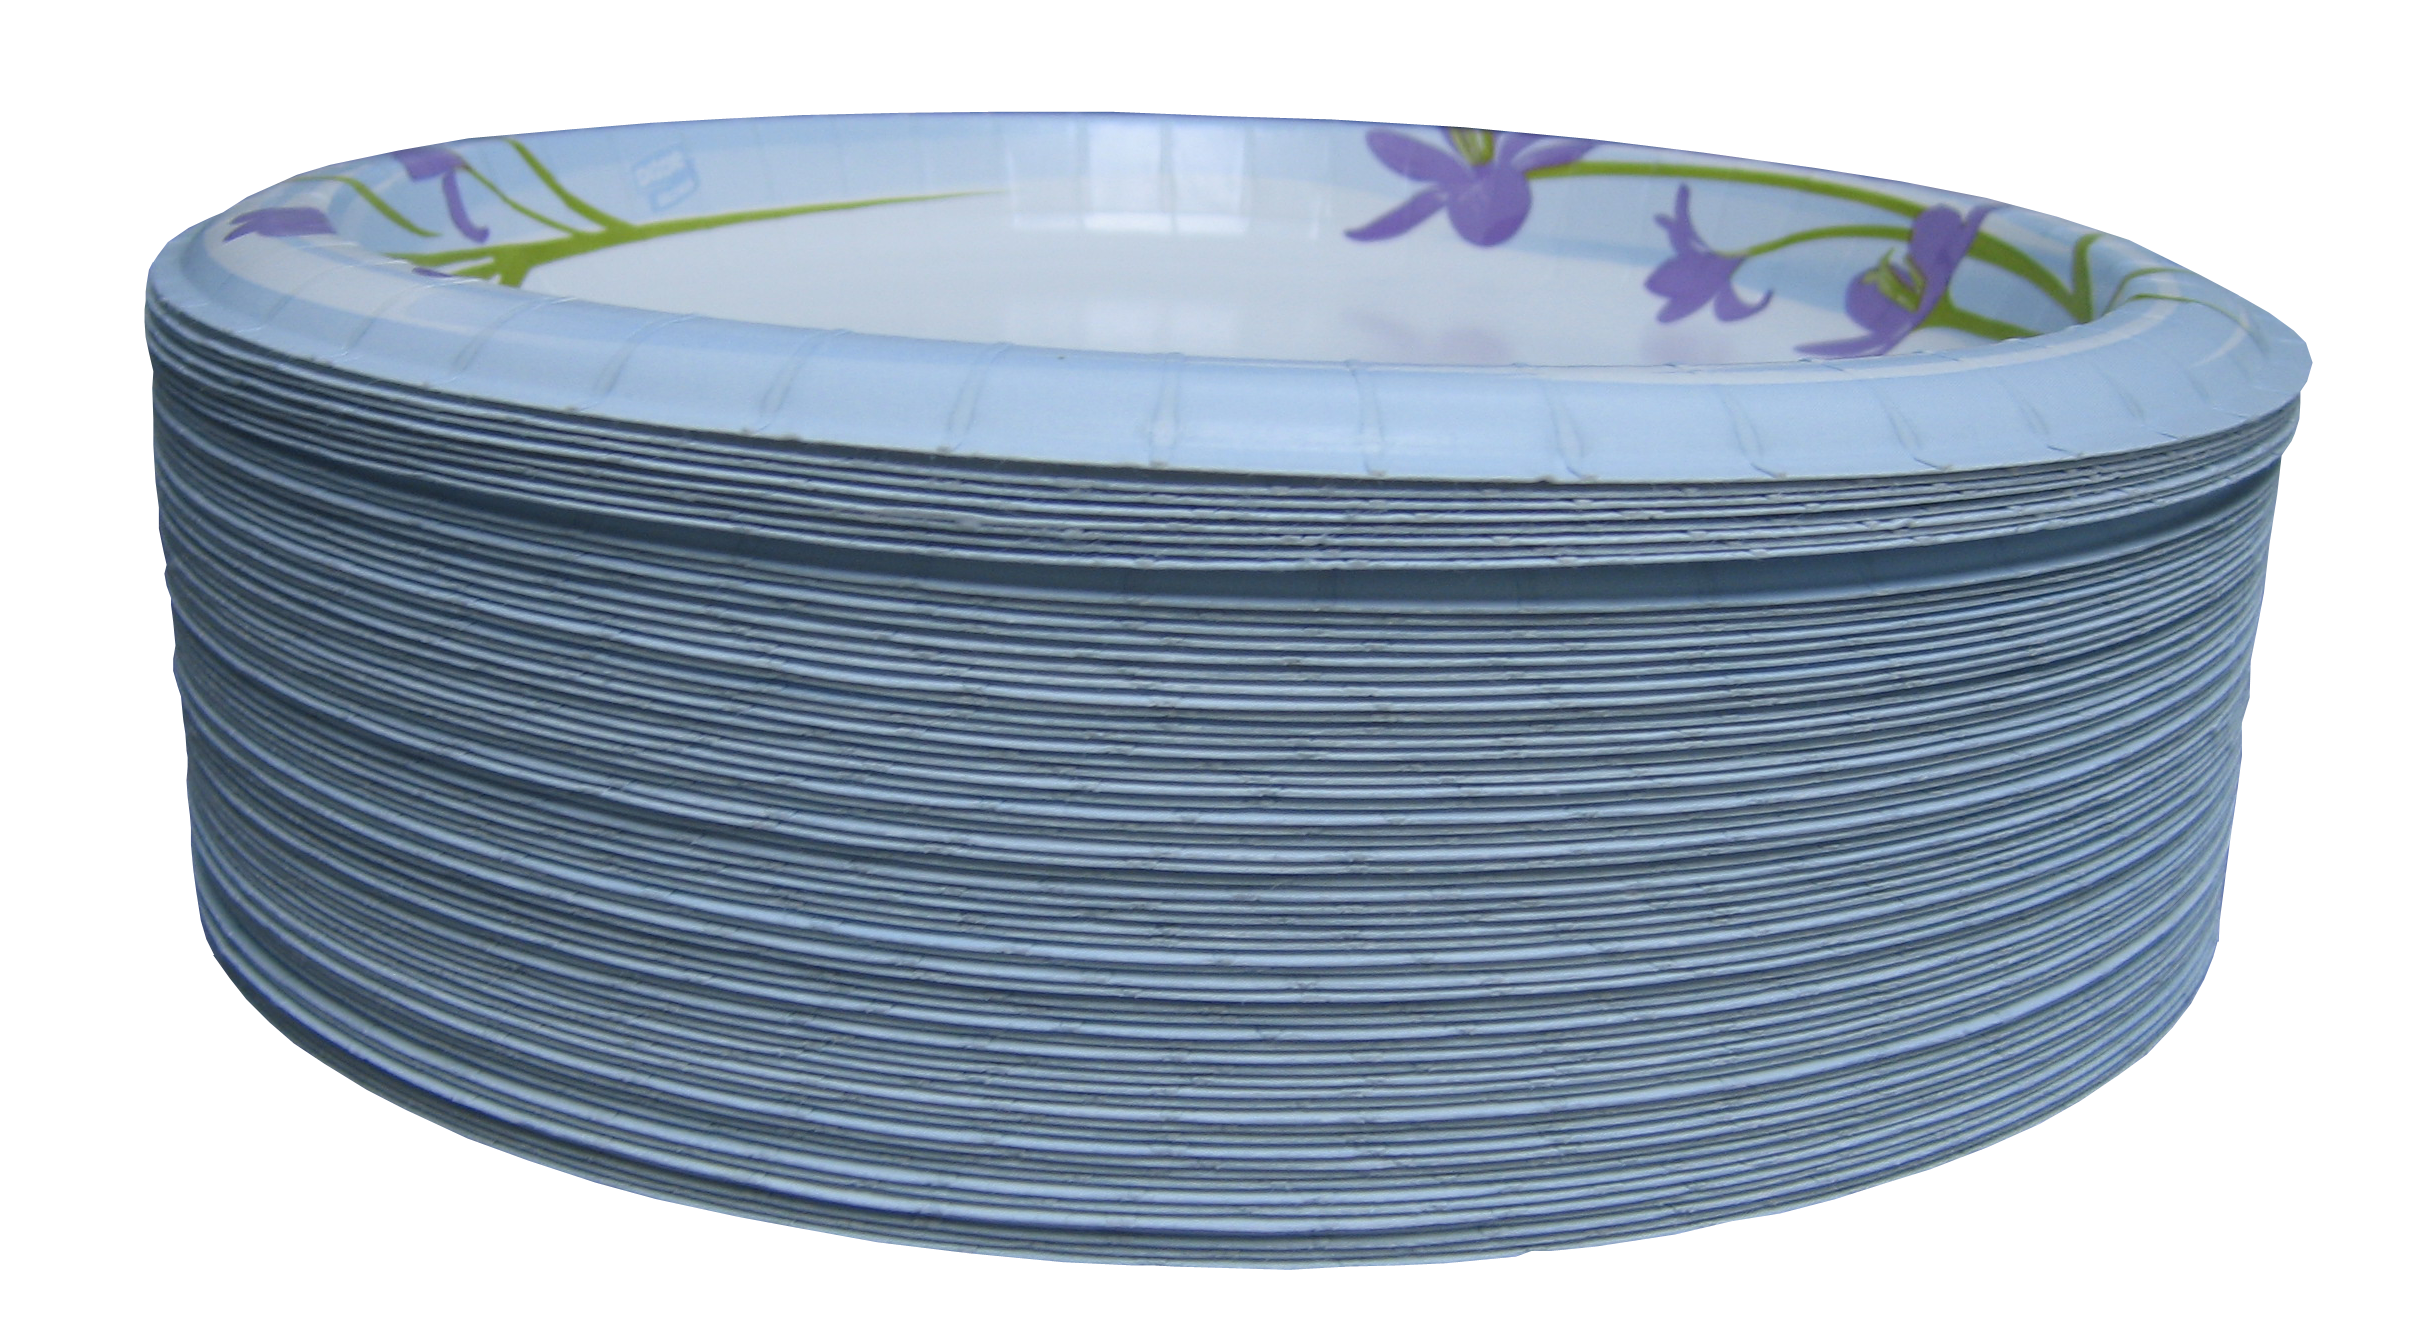
\includegraphics[width=.5\textwidth]{img/stack-of-plates.png}
  \end{center}

  \pause
  \begin{center}
    \begin{tabular}{ccccccc}
      \includegraphics[width=.05\textwidth]{fig/stack-1.pdf}
      &
      remover
      &
      \includegraphics[width=.05\textwidth]{fig/stack-2.pdf}
      &
      inserir 25
      &
      \includegraphics[width=.05\textwidth]{fig/stack-3.pdf}
      &
      inserir 9
      &
      \includegraphics[width=.05\textwidth]{fig/stack-4.pdf}
    \end{tabular}
  \end{center}

\end{frame}

\begin{frame}
  \frametitle{Interface}
  \framesubtitle{Pilhas}

  \begin{itemize}
    \item Tipos
      \begin{itemize}
        \item chave, dado, coleção
      \end{itemize}
    \item Operações
      \begin{itemize}
        \item Inserção (\textit{push\/})
          \begin{itemize}
            \item falha em pilha cheia
          \end{itemize}
        \item Remoção (\textit{pop\/})
          \begin{itemize}
            \item elemento mais recentemente inserido (\textit{LIFO\/})
            \item falha em pilha vazia
          \end{itemize}
        \item Acesso  (\textit{top\/})
          \begin{itemize}
            \item elemento mais recentemente inserido
            \item falha em pilha vazia
          \end{itemize}
        \item Consultas ao estado
          \begin{itemize}
          \item vazia
          \item cheia
          \end{itemize}
      \end{itemize}
  \end{itemize}
\end{frame}

\begin{frame}

  \frametitle{Implementação}
  \framesubtitle{Pilhas}

  \begin{codebox}
    \zi \attrib{P}{Data} \> \> \> \Comment arranjo com os elementos na pilha
    \zi \attrib{P}{Num}  \> \> \> \Comment número de elementos na pilha
    \zi \attrib{P}{Size} \> \> \> \Comment número máximo de elementos na pilha
    \zi $0 \le \attrib{P}{Num} \le \attrib{P}{Size}$
  \end{codebox}
  As posições de um arranjo são numeradas a partir de 1.
\end{frame}

\begin{frame}
  \frametitle{Simulação}
  \framesubtitle{Pilhas}

  \begin{center}
    \begin{tabular}{cc}
      \includegraphics[width=.5\textwidth]{fig/stack-array-1.pdf}
      \pause
      &
      $\id{Pop}$ \pause
      \\
      \includegraphics[width=.5\textwidth]{fig/stack-array-2.pdf}
      \pause
      &
      $\id{Push}(25)$ \pause
      \\
      \includegraphics[width=.5\textwidth]{fig/stack-array-3.pdf}
      \pause
      &
      $\id{Push}(9)$ \pause
      \\
      \includegraphics[width=.5\textwidth]{fig/stack-array-4.pdf}
      &
      $\id{Pop}$ \pause
      \\
      \includegraphics[width=.5\textwidth]{fig/stack-array-5.pdf}
      &
    \end{tabular}
  \end{center}

\end{frame}

\begin{frame}

  \frametitle{Implementação}
  \framesubtitle{Pilhas}

\begin{tabular}{cc}
\begin{minipage}{.42\textwidth}
\begin{codebox}
\Procname{$\proc{Init}(P)$}
\li $\attrib{P}{Num} \gets 0$
\end{codebox}
\pause
\begin{codebox}
\Procname{$\proc{Empty}(P)$}
\li  \Return $\attrib{P}{Num} \isequal 0$
\end{codebox}
\pause
\begin{codebox}
\Procname{$\proc{Full}(P)$}
\li  \Return $\attrib{P}{Num} \isequal \attrib{P}{Size}$
\end{codebox}
\pause
\end{minipage}
&
\begin{minipage}{.55\textwidth}
\begin{codebox}
\Procname{$\proc{Top}(P)$}
\li  \If $\attrib{P}{Num} > 0$
\li    \Then \Return $\attrib{P}{Data}[\attrib{P}{Num}]$
     \End
\end{codebox}
\pause
\begin{codebox}
\Procname{$\proc{Push}(P, v)$}
\li  \If $\attrib{P}{Num} < \attrib{P}{Size}$
\li    \Then $\attrib{P}{Num} \gets \attrib{P}{Num} + 1$
\li      $\attrib{P}{Data}[\attrib{P}{Num}] \gets v$
     \End
\end{codebox}
\pause
\begin{codebox}
\Procname{$\proc{Pop}(P)$}
\li  \If $\attrib{P}{Num} > 0$
\li    \Then $\attrib{P}{Num} \gets \attrib{P}{Num} - 1$
     \End
\end{codebox}
\end{minipage}
\end{tabular}
\end{frame}

\begin{frame}
  \frametitle{Opcionais}
  \framesubtitle{Pilhas}

  \begin{itemize}
    \item Tipos
      \begin{itemize}
        \item iterador
      \end{itemize}
    \item Operações
      \begin{itemize}
        \item acesso à primeira posição da pilha;
        \item acesso à última posição da pilha;
        \item tamanho da pilha.
      \end{itemize}
    \item Implementação
      \begin{itemize}
        \item Redimensionamento dinâmico da capacidade
      \end{itemize}
  \end{itemize}
\end{frame}

\section{Filas}

\begin{frame}
  \frametitle{Filas}

  \begin{center}
    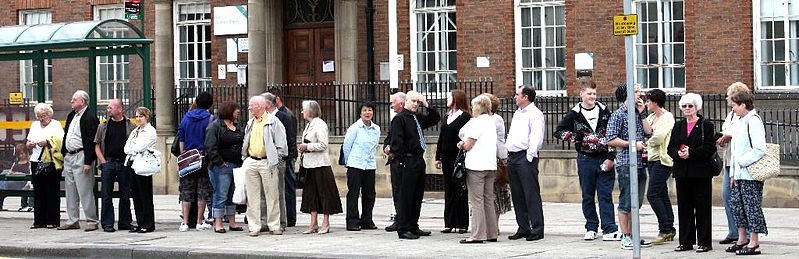
\includegraphics[width=.8\textwidth]{img/queue.jpg}
  \end{center}
  \pause
  \begin{center}
    \begin{tabular}{cc}
      & $\langle 34, 12, 41, 37 \rangle$
      \\
      remover 
      \pause
      & $\langle 12, 41, 37 \rangle$
      \\
      inserir 25
      \pause
      & $\langle 12, 41, 37, 25 \rangle$
      \\
      inserir 9
      \pause
      & $\langle 12, 41, 37, 25, 9 \rangle$
      \\
      remover
      \pause
      & $\langle 41, 37, 25, 9 \rangle$
    \end{tabular}
  \end{center}

\end{frame}

\begin{frame}
  \frametitle{Interface}
  \frametitle{Filas}

  \begin{itemize}
    \item Tipos
      \begin{itemize}
        \item chave, dado, coleção
      \end{itemize}
    \item Operações
      \begin{itemize}
        \item Inserção (\textit{enqueue\/})
          \begin{itemize}
            \item falha em fila cheia
          \end{itemize}
        \item Remoção (\textit{dequeue\/})
          \begin{itemize}
            \item elemento com mais tempo na fila (\textit{LIFO\/})
            \item falha em fila vazia
          \end{itemize}
        \item Acesso  (\textit{head\/})
          \begin{itemize}
            \item elemento com mais tempo na fila
            \item falha em pilha vazia
          \end{itemize}
        \item Consultas ao estado
          \begin{itemize}
          \item vazia
          \item cheia
          \end{itemize}
      \end{itemize}
  \end{itemize}
\end{frame}

\begin{frame}

  \frametitle{Implementação}
  \framesubtitle{Filas}

  \begin{codebox}
    \zi \attrib{Q}{Data} \> \> \> \Comment arranjo com os elementos na pilha
    \zi \attrib{Q}{Hd}   \> \> \> \Comment posição do primeiro elemento
    \zi \attrib{Q}{Tl}   \> \> \> \Comment posição do próximo elemento a entrar
    \zi \attrib{P}{Size} \> \> \> \Comment número máximo de elementos na pilha
    \zi $1 \le \attrib{Q}{Tl} \le \attrib{Q}{Size}$
    \zi $1 \le \attrib{Q}{Hd} \le \attrib{Q}{Size}$
    \zi $\attrib{Q}{Hd} \neq \attrib{Q}{Tl}$
  \end{codebox}
  \begin{itemize}
  \item Posições ocupadas: $\attrib{Q}{Hd}, \attrib{Q}{Hd}+1, \ldots
  \attrib{Q}{Tl}-1$.
  \item No máximo: a capacidade é $\attrib{Q}{Size} - 1$.
  \end{itemize}
  
\end{frame}

\begin{frame}
  \frametitle{Simulação}
  \framesubtitle{Filas}

  \begin{center}
    \begin{tabular}{ccc}
      $\langle 67, 62, 58 \rangle$ &
      \includegraphics[width=.5\textwidth]{fig/queue-array-1.pdf}
      \pause
      &
      $\id{Dequeue}$ \pause
      \\
      $\langle 62, 58 \rangle$ &
      \includegraphics[width=.5\textwidth]{fig/queue-array-2.pdf}
      \pause
      &
      $\id{Enqueue}(25)$ \pause
      \\
      $\langle 62, 58, 25 \rangle$ &
      \includegraphics[width=.5\textwidth]{fig/queue-array-3.pdf}
      \pause
      &
      $\id{Enqueue}(25)$ \pause
      \\
      $\langle 62, 58, 25, 9 \rangle$ &
      \includegraphics[width=.5\textwidth]{fig/queue-array-4.pdf}
      &
      $\id{Dequeue}$ \pause
      \\
      $\langle 58, 25, 9 \rangle$ &
      \includegraphics[width=.5\textwidth]{fig/queue-array-5.pdf}
      &
    \end{tabular}
  \end{center}

\end{frame}

\begin{frame}

  \frametitle{Implementação}
  \framesubtitle{Filas}

\begin{codebox}
\Procname{$\proc{Init}(Q)$}
\li $\attrib{Q}{Hd} \gets 1$
\li $\attrib{Q}{Tl} \gets 1$
\end{codebox}
\begin{codebox}
\Procname{$\proc{Empty}(Q)$}
\li  \Return $\attrib{Q}{Hd} \isequal \attrib{Q}{Tl}$
\end{codebox}
\begin{codebox}
\Procname{$\proc{Full}(Q)$}
\li  \Return $\attrib{Q}{Hd} \isequal \attrib{Q}{Tl} + 1$ or
\li  \> ($\attrib{Q}{Hd} \isequal 1$ and $\attrib{Q}{Hd} \isequal \attrib{Q}{Size}$)
\end{codebox}

\end{frame}

\begin{frame}

  \frametitle{Implementação}
  \framesubtitle{Filas}

\begin{codebox}
\Procname{$\proc{Head}(Q)$}
\li  \If not $\proc{Empty}(Q)$
\li    \Then \Return $\attrib{Q}{Data}[\attrib{Q}{Hd}]$
     \End
\end{codebox}
\begin{codebox}
\Procname{$\proc{Enqueue}(Q, v)$}
\li  \If not $\proc{Full}(Q)$
\li    \Then $\attrib{Q}{Data}[\attrib{Q}{Tl}] \gets v$
\li      $\attrib{Q}{Tl} \gets 1 + (\attrib{Q}{Tl} \mod \attrib{Q}{Size})$
     \End
\end{codebox}
\begin{codebox}
\Procname{$\proc{Dequeue}(Q)$}
\li  \If not $\proc{Empty}(Q)$
\li    \Then $\attrib{Q}{Hd} \gets 1 + (\attrib{Q}{Hd} \mod \attrib{Q}{Size})$
     \End
\end{codebox}

\end{frame}

\begin{frame}
  \frametitle{Opcionais}
  \framesubtitle{Fila}

  \begin{itemize}
    \item Tipos
      \begin{itemize}
        \item iterador
      \end{itemize}
    \item Operações
      \begin{itemize}
        \item acesso à primeira posição da fila;
        \item acesso à última posição da fila;
        \item tamanho da fila.
      \end{itemize}
    \item Implementação
      \begin{itemize}
        \item Redimensionamento dinâmico da capacidade
      \end{itemize}
  \end{itemize}
\end{frame}

\section{Filas de duas entradas}

\begin{frame}
  \frametitle{Filas de duas entradas}

  \begin{itemize}

    \item \textit{Double-ended queue\/} (\textit{deque\/});
     
    \item inserção e remoção nas duas pontas da fila;

    \item acesso aos elementos nas pontas da fila;

    \item pode ser usada para representar fila e pilha.

  \end{itemize}
\end{frame}

\begin{frame}
  \frametitle{Interface}
  \frametitle{Deque}

  \begin{itemize}
    \item Tipos
      \begin{itemize}
        \item chave, dado, coleção
      \end{itemize}
    \item Operações
      \begin{itemize}
        \item Inserção na cabeça (\textit{push\_front\/}) e na cauda (\textit{push\_back\/})
          \begin{itemize}
            \item falha em fila cheia
          \end{itemize}
        \item Remoção na cabeça (\textit{pop\_front\/}) e na cauda (\textit{pop\_back\/})
          \begin{itemize}
            \item falha em fila vazia
          \end{itemize}
        \item Acesso na cabeça (\textit{front\/}) e na cauda (\textit{back\/})
          \begin{itemize}
            \item falha em pilha vazia
          \end{itemize}
        \item Consultas ao estado
          \begin{itemize}
          \item vazia
          \item cheia
          \end{itemize}
      \end{itemize}
  \end{itemize}
\end{frame}

\begin{frame}

  \frametitle{Implementação}
  \framesubtitle{Deque}

  \begin{codebox}
    \zi \attrib{Q}{Data} \> \> \> \Comment arranjo com os elementos na pilha
    \zi \attrib{Q}{Hd}   \> \> \> \Comment posição do primeiro elemento
    \zi \attrib{Q}{Tl}   \> \> \> \Comment posição do próximo elemento a entrar
    \zi \attrib{P}{Size} \> \> \> \Comment número máximo de elementos na pilha
    \zi $1 \le \attrib{Q}{Tl} \le \attrib{Q}{Size}$
    \zi $1 \le \attrib{Q}{Hd} \le \attrib{Q}{Size}$
    \zi $\attrib{Q}{Hd} \neq \attrib{Q}{Tl}$
  \end{codebox}
  \begin{itemize}
  \item Posições ocupadas: $\attrib{Q}{Hd}, \attrib{Q}{Hd}+1, \ldots
  \attrib{Q}{Tl}-1$.
  \item No máximo: a capacidade é $\attrib{Q}{Size} - 1$.
  \end{itemize}
  
\end{frame}

\begin{frame}
  \frametitle{Simulação}
  \framesubtitle{Filas}

  \begin{center}
    \begin{tabular}{ccc}
      $\langle 67, 62, 58 \rangle$ &
      \includegraphics[width=.45\textwidth]{fig/deque-array-1.pdf}
      \pause
      &
      $\id{Pop-Front}$ \pause
      \\
      $\langle 62, 58 \rangle$ &
      \includegraphics[width=.45\textwidth]{fig/deque-array-2.pdf}
      \pause
      &
      $\id{Pop-Back}$ \pause
      \\
      $\langle 62 \rangle$ &
      \includegraphics[width=.45\textwidth]{fig/deque-array-3.pdf}
      \pause
      &
      $\id{Push-Front}(9)$ \pause
      \\
      $\langle 9, 62 \rangle$ &
      \includegraphics[width=.45\textwidth]{fig/deque-array-4.pdf}
      &
      $\id{Push-Back}(25)$ \pause
      \\
      $\langle 9, 62, 25 \rangle$ &
      \includegraphics[width=.45\textwidth]{fig/deque-array-5.pdf}
      &
    \end{tabular}
  \end{center}

\end{frame}

\begin{frame}

  \frametitle{Implementação}
  \framesubtitle{Deque}

\begin{codebox}
\Procname{$\proc{Init}(Q)$}
\li $\attrib{Q}{Hd} \gets 1$
\li $\attrib{Q}{Tl} \gets 1$
\end{codebox}
\begin{codebox}
\Procname{$\proc{Empty}(Q)$}
\li  \Return $\attrib{Q}{Hd} \isequal \attrib{Q}{Tl}$
\end{codebox}
\begin{codebox}
\Procname{$\proc{Full}(Q)$}
\li  \Return $\attrib{Q}{Hd} \isequal \attrib{Q}{Tl} + 1$ or
\li  \> ($\attrib{Q}{Hd} \isequal 1$ and $\attrib{Q}{Hd} \isequal \attrib{Q}{Size}$)
\end{codebox}

\end{frame}

\begin{frame}

  \frametitle{Implementação}
  \framesubtitle{Deque}

\begin{codebox}
\Procname{$\proc{Front}(Q)$}
\li  \If not $\proc{Empty}(Q)$
\li    \Then \Return $\attrib{Q}{Data}[\attrib{Q}{Hd}]$
     \End
\end{codebox}
\begin{codebox}
\Procname{$\proc{Push-Back}(Q, v)$}
\li  \If not $\proc{Full}(Q)$
\li    \Then $\attrib{Q}{Data}[\attrib{Q}{Tl}] \gets v$
\li      $\attrib{Q}{Tl} \gets 1 + (\attrib{Q}{Tl} \mod \attrib{Q}{Size})$
     \End
\end{codebox}
\begin{codebox}
\Procname{$\proc{Pop-Front}(Q)$}
\li  \If not $\proc{Empty}(Q)$
\li    \Then $\attrib{Q}{Hd} \gets 1 + (\attrib{Q}{Hd} \mod \attrib{Q}{Size})$
     \End
\end{codebox}

\end{frame}

\begin{frame}

  \frametitle{Implementação}
  \framesubtitle{Deque}

\begin{codebox}
\Procname{$\proc{Back}(Q)$}
\li  \If not $\proc{Empty}(Q)$
\li    \Then \Return $\attrib{Q}{Data}[\attrib{Q}{Tl}]$
     \End
\end{codebox}
\begin{codebox}
\Procname{$\proc{Push-Front}(Q, v)$}
\li  \If not $\proc{Full}(Q)$
\li    \Then $\attrib{Q}{Data}[\attrib{Q}{Hd}] \gets v$
\li      \If $\attrib{Q}{Hd} \isequal 1$
\li        \Then $\attrib{Q}{Hd} \gets \attrib{Q}{Size}$
\li        \Else $\attrib{Q}{Hd} \gets \attrib{Q}{Hd} - 1$
         \End
     \End
\end{codebox}
\begin{codebox}
\Procname{$\proc{Pop-Back}(Q)$}
\li  \If not $\proc{Empty}(Q)$
\li    \Then \If $\attrib{Q}{Tl} \isequal 1$
\li      \Then $\attrib{Q}{Tl} \gets \attrib{Q}{Size}$
\li      \Else $\attrib{Q}{Tl} \gets \attrib{Q}{Hd} - 1$
       \End
     \End
\end{codebox}

\end{frame}

\begin{frame}

  \frametitle{Exercícios}

  \begin{itemize}

    \item É possível implementar as funcionalidades de fila utilizando pilha(s)?
      Se sim, como? Se não, por que?

    \item É possível implementar as funcionalidades de pilha utilizando fila(s)?
      Se sim, como? Se não, por que?

    \item É possível implementar as funcionalidades de deque utilizando pilha(s)
      e fila(s)?  Se sim, como? Se não, por que?

  \end{itemize}
\end{frame}
%% \section{Listas encadeadas}

%% \begin{frame}
%%   \frametitle{Listas encadeadas}
%% \end{frame}

%% \section{Encadeamento em arranjos}

%% \begin{frame}
%%   \frametitle{Registros e encadeamento com arranjos}
%% \end{frame}

\end{document}

